This section looks at previous work in similar fields. It starts with presenting the paper that presents the idea that this thesis further explores, and then looks at past research on using Twitter and critical infrastructure data for similar tasks.

\section{Spatiotemporal information from urban systems}
In the novel study of "Detecting flu outbreaks based on spatiotemporal information from an urban system", which is the base idea for this thesis, Grottenberg et al. \cite{spatiotemp_urban_sys} outlines a design for a system for surveillance of flu outbreaks. Emphasis on the belief that real-time data flows could prove useful in both understanding social functions during disasters and crisis as well as give " ... actionable intelligence for use in influenza management efforts.".
The borrowed figure \ref{fig:grottenberg} from his article sums up what this thesis hopes to accomplish, namely to find a correlation between different datasets and the datasets from the Norwegian public health institution (NIPH), this interference of public behaviour would become visible in essential criterion.
This short read \cite{spatiotemp_urban_sys} is recommended as it gives a more in-depth understanding of the incentive for this thesis

\begin{figure}[h]
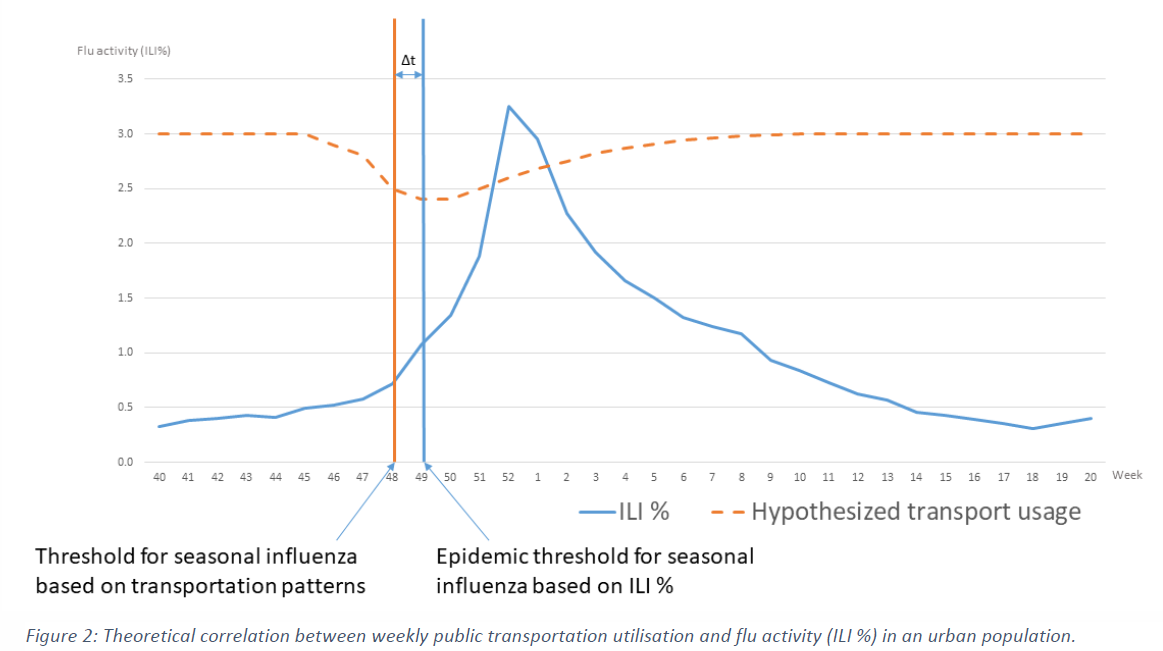
\includegraphics[width=16cm]{grottenberg}
\centering
\caption{Figure from Grottenberg et al. \cite{spatiotemp_urban_sys}}
\label{fig:grottenberg}
\end{figure}

\section{Twitter}
A number of studies have been created on the information users on Twitter generate in providing valuable insights into the population by analysing millions of twitter messages (tweets). Researchers have studied tweets to reveal political opinions\cite{twitter_politic}, measure public health\cite{twitter_flu_trends}, linguistic sentiments\cite{twitter_linguistics} and even environmental phenomena such as earthquakes\cite{twitter_earthQuake}. Achrekar et al.\cite{twitter_flu_trends} examines tweet flu trends and compares them with actual influenza data. The results show a high correlation between self-reported instances of flu-like illnesses (ILI) and reported ILI by public health providers. Achrekar references claims that early prevention limits the spread of infectious diseases and that twitter data is an 'untapped data source' that actually is quite reliable. This demonstrates how social media can be  used to predict real-world consequences, and gives credibility to usage in this thesis. \\Michal J. Paul and Mark Dredze \cite{twitter_what_you_tweet} also conducted research on the usage of twitter data to measure population characteristics. In their conclusion twitter data from many users divulges reliable information about a certain topic of interest and in particular public health. They further discuss the pros and cons namely that self-reported is low cost and rapid transmission, whereas on the other side this is a 'blind authorship, lack of source citation and presentation of opinion as fact'. Certainly twitter messages may be false on an individual level, but however when taking into account thousands or even millions of messages this seems not plausible on a bigger scale. Albuquerque et al. \cite{de2015geographic} describes how they were able to extract useful information via twitter to better acquire information about a flood phenomena in German rivers, and combining this with authoritative data for disaster management. They write that social media messages gives a valuable and useful information to manage disasters, in a way this is practically the same as asking volunteers for help. For these reasons twitter data is used in this thesis as it proves an interesting and unique source of relevant information.

\section{Data management and critical infrastructure}
This thesis touches upon data management and development of crisis response systems. The proposed system would act as a tool in a larger system in the development of support decision making in the event of a epidemic influenza preparedness and outbreak. 

Responding to extensive crisis or disasters requires coordination between a multitude of relief agencies, and this demands the right information at the right time. A system that can detect an emergence of a possible influenza outbreak would be an aiding factor to this. Gonzales et al. \cite{gonzalez2009framework} goes into general details of how the quality of information during a crisis response is important and how to better coordinate relief agencies with the right information at the right time. They conclude that designing a computer based system for management and automation services of a work flow information conductor would better the over all quality of response and guidance. The system proposed by this thesis could be a module of such a system. Simulation modules could also be added to this system. This thesis is not a simulation tool but it is worth mentioning that there are several such proposed models of influenza and other disease simulation implementations. Shao et al. \cite{shao2016forecasting} ask the question of whether it is possible by monitoring public urban data to predict the coming outline of an overall epidemic, and simulates this. There are many more simulation tools, another is proposed by Stein et al. \cite{stein2012development} which models an influenza outbreak in two provinces of Lao. Simulations are a way of preparing and training in order to reveal flaws and evaluation of response plans and deployment of limited health care resources.
